\begin{frame}{Proof Systems}

	$L \subseteq \{0, 1\}^*$. $\UNSAT$ is a language of unsatisfiable boolean CNF formulas.
    \pause

    \begin{definition}[Cook, Reckhow 79]
        Proof system for $L \Leftrightarrow$ poly-time algorithm
        $\Pi\colon \{0, 1\}^* \times \{0, 1\}^* \rightarrow \{0, 1\}$:
        \begin{itemize}
            \item (completeness) $x \in L \Rightarrow \exists w ~ \Pi(x, w) = 1$;
            \item (soundness) $\exists w ~ \Pi(x, w) = 1 \Rightarrow x \in L$.
        \end{itemize}
    \end{definition}

    Length of $|w|$ is the complexity measure.

    \pause

    \begin{block}{Cook's Program}
        Prove superpolynomial lower bounds for stronger and stronger proof systems until the techniques
        are developed to do it in a general case.

        Goal: $\NP \neq \coNP$.
    \end{block}
\end{frame}

\begin{frame}{Proof Systems}

    \deftext{Resolution}: proof of $\varphi \coloneqq \bigwedge\limits_{i} C_i$ is a sequence of clauses
    $(D_1, D_2, D_3, \dots, D_{\ell})$:
    \pause
    
    \begin{minipage}{0.3\linewidth}
        \begin{itemize}
            \item $D_i \in \{C_i\}$;
                \pause
            \item $\frac{A \lor x ~~~~~ B \lor \bar{x}}{A \lor B}$, $D_i \coloneqq A \lor B$;
                \pause
            \item $D_{\ell} = \emptyset$.
        \end{itemize}
    \end{minipage}
    \pause
    \begin{minipage}{0.68\linewidth}
        \centering
        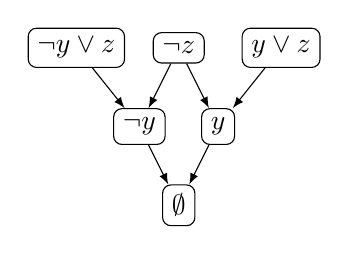
\begin{tikzpicture}[>=latex]
    \node[rectangle, rounded corners = 3pt, draw] (a) at (-1.3, 2)
        {$\neg y \lor z$};
    \node[rectangle, rounded corners = 3pt, draw] (a2) at (1.3, 2)
        {$y \lor z$};
    \node[rectangle, rounded corners = 3pt, draw] (b) at (0, 2)
        {$\neg z$};
    \node[rectangle, rounded corners = 3pt, draw] (c) at (-0.5, 1)
        {$\neg y$};
    \node[rectangle, rounded corners = 3pt, draw] (d) at (0.5, 1)
       {$y$};
    \node[rectangle, rounded corners = 3pt, draw] (e) at (0, 0)
        {$\emptyset$};

    \draw[->] (a) -- (c);
    \draw[->] (a2) -- (d);
    \draw[->] (b) -- (c);
    \draw[->] (b) -- (d);
    \draw[->] (c) -- (e);
    \draw[->] (d) -- (e);
\end{tikzpicture}
    \end{minipage}


    \pause
    \vspace{0.3cm}

    \deftext{Cutting Planes}: proof is a sequence of inequalities over $\mathbb{Z}$
    $(p_1 \ge 0, p_2 \ge 0, p_3 \ge 0, \dots, p_{\ell} \ge 0)$:
    \begin{itemize}
        \item $p_i$ is an encoding of $C \in \varphi$, $x_k \ge 0$ or $-x_k + 1 \ge 0$;
        \item $\frac{p_i ~~~~~ p_j}{p_k}$,  $(p_i \ge 0) \land (p_j \ge 0)$ imply $(p_k \ge 0)$
            \alert{over $\mathbb{Z}^n$};
        \item $p_{\ell} = 1$.
    \end{itemize}

    \pause
    \vspace{0.3cm}

    \deftext{Nullstellensatz}: proof of a system of polynomial equalities $f_1 = 0, f_2 = 0, \dots$:
    $$
        \sum_{u = 1}^{a} p_u f_u = 1.
    $$
\end{frame}


\begin{frame}{Pebbing}

    \begin{center}
        \tikzstyle{vert} = [
    circle,
    draw,
    inner sep = 0pt,
    minimum size = 0.45cm,
    fill = LEIorange!5
]
\tikzstyle{pstyle} = [alt = <{#1}>{fill = LEIorange!50}{}]
    
\tikzset{
    xcenter around/.style 2 args = {
        execute at end picture = {%
            \useasboundingbox let \p0 = (current bounding box.south west),
            \p1 = (current bounding box.north east),
            \p2 = (#1),
            \p3 = (#2) in ({min(\x2 + \x3 - \x1, \x0)}, \y0) rectangle ({max(\x3 + \x2 - \x0, \x1)},\y1);
        }
    }
}

\begin{tikzpicture}[xcenter around = {-2.1, -2.1}{2.1, 0.1}]
    \node at (3.6, -0.6) {
\includegraphics[scale = 0.09]{pics/utia-rest.png}};
    
    \node[vert, pstyle = 2, pstyle = {9-}, alt = <10>{fill = red!60}{}] (a) at (0, 0) {$r$};
    \node[vert, pstyle = 4, pstyle = {7-}] (b) at (-1, -1) {$x$};
    \node[vert, pstyle = {8-}] (c) at (1, -1) {$y$};
    \node[vert, pstyle = {3-4}, pstyle = {6-}] (d) at (-2, -2) {$z$};
    \node[vert, pstyle = {3-4}, pstyle = {6-}] (e) at (0, -2) {$u$};
    \node[vert, pstyle = 3, pstyle = {8-}] (f) at (2, -2) {$w$};

    \draw[->] (b) -- (a);
    \draw[->] (c) -- (a);
    \draw[->] (d) -- (b);
    \draw[->] (e) -- (b);
    \draw[->] (e) -- (c);
    \draw[->] (f) -- (c);
\end{tikzpicture}        
    \end{center}

    \pause
    \begin{itemize}
        \item $(\neg r)$;
            \pause
        \item $(z), (u), (w)$;
            \pause
        \item $(\neg z \lor \neg u \lor x)$.    
    \end{itemize}

    \pause
    \tikzset{
    pr-vert/.style = {
        draw,
        rounded rectangle,
        minimum width = 1cm,
        minimum height = 0.4cm,
        outer sep = 0pt,
        fill = #1
    },
    pr-vert/.default = LEIblue!10
}

\tikzstyle{ops} = [alt = <{#1-}>{opacity = 1}{opacity = 0}]

\begin{tikzpicture}
    \node[pr-vert, ops = 6] (a) at (0, 0) {$u$};
    \node[pr-vert, ops = 6] (b) at (0, -1) {$z$};
    \node[pr-vert, ops = 6] (c) at (0, -2) {$\neg z \lor \neg u \lor x$};
    
    \node[pr-vert = LEIorange!10, ops = 7] (d) at (2, -1.9) {$\neg u \lor x$};
    \node[pr-vert = LEIorange!10, ops = 7] (e) at (3, -1.25) {$x$};

    \node[pr-vert, ops = 8] (f) at (4, 0) {$\neg u \lor \neg w \lor y$};
    \node[pr-vert, ops = 8] (g) at (6, 0) {$w$};
    
    \node[pr-vert = LEIorange!10, ops = 8] (h) at (5, -0.75) {$\neg w \lor y$};
    \node[pr-vert = LEIorange!10, ops = 8] (i) at (6.5, -1) {$y$};

    \node[pr-vert, ops = 9] (j) at (5, -2) {$\neg x \lor \neg y \lor r$};

    \node[pr-vert = LEIorange!10, ops = 9] (k) at (7.5, -2) {$\neg y \lor r$};
    \node[pr-vert = LEIorange!10, ops = 9] (l) at (8.5, -1.2) {$r$};

    \node[pr-vert, ops = 10] (m) at (8.5, 0) {$\neg r$};

    \node[pr-vert = red!30, ops = 10] (n) at (9.5, -0.6) {$\emptyset$};

    \draw[->, ops = 7] (b) -- (d);
    \draw[->, ops = 7] (c) -- (d);
    \draw[->, ops = 7] (a) -- (e);
    \draw[->, ops = 7] (d) -- (e);

    \draw[->, ops = 8] (a) -- (h);
    \draw[->, ops = 8] (f) -- (h);
    \draw[->, ops = 8] (h) -- (i);
    \draw[->, ops = 8] (g) -- (i);

    \draw[->, ops = 9] (e) -- (k);
    \draw[->, ops = 9] (j) -- (k);
    \draw[->, ops = 9] (k) -- (l);
    \draw[->, ops = 9] (i) -- (l);

    \draw[->, ops = 10] (l) -- (n);
    \draw[->, ops = 10] (m) -- (n);
\end{tikzpicture}
\end{frame}

\begin{frame}{$\DPLL$ Algorithms}

    \begin{center}
        \begin{frame}

    \begin{center}
        \Huge Part II: SAT Solving and Proof Complexity
    \end{center}
    
\end{frame}

\begin{frame}{$\DPLL$ Algorithms}

    \begin{center}
        \begin{frame}

    \begin{center}
        \Huge Part II: SAT Solving and Proof Complexity
    \end{center}
    
\end{frame}

\begin{frame}{$\DPLL$ Algorithms}

    \begin{center}
        \begin{frame}

    \begin{center}
        \Huge Part II: SAT Solving and Proof Complexity
    \end{center}
    
\end{frame}

\begin{frame}{$\DPLL$ Algorithms}

    \begin{center}
        \input{pics/dpll.tex}        
    \end{center}

    
	\pause
    \pause
    \pause
    \pause
    \pause
    \begin{itemize}
        \item Heuristic $\mathbf{A}$ chooses a variable for splitting.
    	\pause
	    \item Heuristic $\mathbf{B}$ chooses the first value.
    	\pause
    	\item Simplification rules: \alert{no simplifications!}
    \end{itemize}
\end{frame}

\begin{frame}{$\DPLL$ and Resolution}
    
    \begin{theorem}
        $\DPLL$ algoritm makes $t$ splitting on \alert{unsatisfiable} CNF formula
        $$\varphi \coloneqq \bigwedge\limits_i C_i$$
        $\Rightarrow$ there exists a resolution proof of $\varphi$ of size $2t$.
    \end{theorem}

    \pause

    \begin{minipage}{0.58\linewidth}
        \centering
        \input{pics/dpll-2.tex}
    \end{minipage}
    \pause
    \begin{minipage}{0.4\linewidth}
        \centering
        $\frac{A \lor x ~~~ B \lor \neg x}{A \lor B} ~~~~~ \frac{A}{A \lor z}$
        \begin{itemize}
            \item Node $\Rightarrow$ disjunction of negations of queries.
            \item $(x \lor \neg y \lor \neg z \lor u)$.
        \end{itemize}
    \end{minipage}

\end{frame}

\begin{frame}{Corollaries}

    \begin{itemize}
        \item{} Running time of $\DPLL$ on $\PHP_{n}^{n + 1}$ is at least $2^{\Omega(n)}$.
            \pause
        \item{} [Alekhnovich, Hirsch, Itsykson 05; \alert{informal}] Running time of \alert{restricted}
            $\DPLL$ on some \alert{sat. formulas} is at least $2^{\Omega(n)}$. 
    \end{itemize}

    \pause
    \vspace{0.5cm}
    \begin{block}{Remark}
        $\alg{CDCL} \approx$ general resolution.
    \end{block}

    \pause
    \begin{itemize}
        \item{} Running time of $\alg{CDCL}$ on $\PHP_{n}^{n + 1}$ is at least $2^{\Omega(n)}$.
        \item{} \alert{Open problem}: what about sat. formulas and $\alg{CDCL}$?
    \end{itemize}

\end{frame}
        
    \end{center}

    
	\pause
    \pause
    \pause
    \pause
    \pause
    \begin{itemize}
        \item Heuristic $\mathbf{A}$ chooses a variable for splitting.
    	\pause
	    \item Heuristic $\mathbf{B}$ chooses the first value.
    	\pause
    	\item Simplification rules: \alert{no simplifications!}
    \end{itemize}
\end{frame}

\begin{frame}{$\DPLL$ and Resolution}
    
    \begin{theorem}
        $\DPLL$ algoritm makes $t$ splitting on \alert{unsatisfiable} CNF formula
        $$\varphi \coloneqq \bigwedge\limits_i C_i$$
        $\Rightarrow$ there exists a resolution proof of $\varphi$ of size $2t$.
    \end{theorem}

    \pause

    \begin{minipage}{0.58\linewidth}
        \centering
        \tikzstyle{inner} = [circle, minimum size = 0.3cm, draw, inner sep = 0.1pt]
\tikzstyle{gstyle} = [fill = green]
\tikzstyle{rstyle} = [fill = red]
\tikzstyle{ed} = [->, draw]
\tikzstyle{ops} = [alt=<{#1-}>{opacity = 1}{opacity = 0}]
\tikzstyle{opstyle} = [inner, ops = #1]
\tikzstyle{oped} = [ed, ops = #1]
\tikzstyle{gstyle} = [alt=<{#1}>{fill = green}{}]
\tikzstyle{rstyle} = [alt=<{#1}>{red!90!black}{}]
\tikzstyle{snakestyle} = [
    alt=<{#1}>{
        decorate,
        decoration = {
            snake,
            amplitude = 0.4mm,
            segment length = 2mm,
            post length = 1mm
        }
    }{}]


    
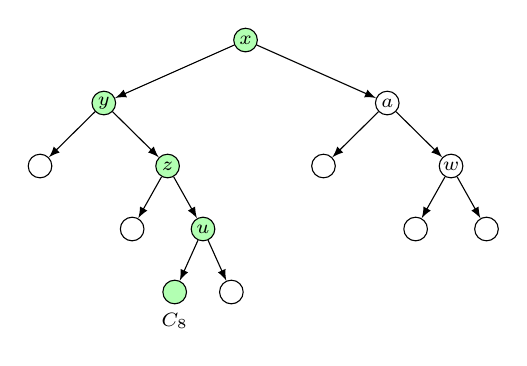
\begin{tikzpicture}[>=latex, xscale = 0.9]
    
    \node[inner, fill = green!30] (a) at (0, 0) {\scriptsize $x$};
    \node[inner, fill = green!30] (b) at (-2, -0.8) {\scriptsize $y$};
    \node[inner] (c) at (2, -0.8) {\scriptsize $a$};
    \node[inner] (d) at (-2.9, -1.6) {};
    \node[inner, fill = green!30] (e) at (-1.1, -1.6) {\scriptsize $z$};
    \node[inner] (f) at (1.1, -1.6) {};
    \node[inner] (g) at (2.9, -1.6) {\scriptsize $w$};

    \node[inner] (h) at (-1.6, -2.4) {};
	\node[inner, fill = green!30] (i) at (-0.6, -2.4) {\scriptsize $u$};
    
    \node[inner] (j) at (2.4, -2.4) {};
    \node[inner] (k) at (3.4, -2.4) {};

    \node[inner, fill = green!30] (l) at (-1, -3.2) {};
    \node[below = 4pt] at (l) {\scriptsize $C_{8}$};
    \node[inner] (m) at (-0.2, -3.2) {};
    
    \draw[ed] (a) -- (b);
    \draw[ed] (a) -- (c);
    \draw[ed] (b) -- (d);
    \draw[ed] (b) -- (e);
    \draw[ed] (c) -- (f);
    \draw[ed] (c) -- (g);
    \draw[ed] (e) -- (h);
    \draw[ed] (e) -- (i);
    \draw[ed] (g) -- (j);
    \draw[ed] (g) -- (k);
    \draw[ed] (i) -- (l);
    \draw[ed] (i) -- (m);
\end{tikzpicture}
    \end{minipage}
    \pause
    \begin{minipage}{0.4\linewidth}
        \centering
        $\frac{A \lor x ~~~ B \lor \neg x}{A \lor B} ~~~~~ \frac{A}{A \lor z}$
        \begin{itemize}
            \item Node $\Rightarrow$ disjunction of negations of queries.
            \item $(x \lor \neg y \lor \neg z \lor u)$.
        \end{itemize}
    \end{minipage}

\end{frame}

\begin{frame}{Corollaries}

    \begin{itemize}
        \item{} Running time of $\DPLL$ on $\PHP_{n}^{n + 1}$ is at least $2^{\Omega(n)}$.
            \pause
        \item{} [Alekhnovich, Hirsch, Itsykson 05; \alert{informal}] Running time of \alert{restricted}
            $\DPLL$ on some \alert{sat. formulas} is at least $2^{\Omega(n)}$. 
    \end{itemize}

    \pause
    \vspace{0.5cm}
    \begin{block}{Remark}
        $\alg{CDCL} \approx$ general resolution.
    \end{block}

    \pause
    \begin{itemize}
        \item{} Running time of $\alg{CDCL}$ on $\PHP_{n}^{n + 1}$ is at least $2^{\Omega(n)}$.
        \item{} \alert{Open problem}: what about sat. formulas and $\alg{CDCL}$?
    \end{itemize}

\end{frame}
        
    \end{center}

    
	\pause
    \pause
    \pause
    \pause
    \pause
    \begin{itemize}
        \item Heuristic $\mathbf{A}$ chooses a variable for splitting.
    	\pause
	    \item Heuristic $\mathbf{B}$ chooses the first value.
    	\pause
    	\item Simplification rules: \alert{no simplifications!}
    \end{itemize}
\end{frame}

\begin{frame}{$\DPLL$ and Resolution}
    
    \begin{theorem}
        $\DPLL$ algoritm makes $t$ splitting on \alert{unsatisfiable} CNF formula
        $$\varphi \coloneqq \bigwedge\limits_i C_i$$
        $\Rightarrow$ there exists a resolution proof of $\varphi$ of size $2t$.
    \end{theorem}

    \pause

    \begin{minipage}{0.58\linewidth}
        \centering
        \tikzstyle{inner} = [circle, minimum size = 0.3cm, draw, inner sep = 0.1pt]
\tikzstyle{gstyle} = [fill = green]
\tikzstyle{rstyle} = [fill = red]
\tikzstyle{ed} = [->, draw]
\tikzstyle{ops} = [alt=<{#1-}>{opacity = 1}{opacity = 0}]
\tikzstyle{opstyle} = [inner, ops = #1]
\tikzstyle{oped} = [ed, ops = #1]
\tikzstyle{gstyle} = [alt=<{#1}>{fill = green}{}]
\tikzstyle{rstyle} = [alt=<{#1}>{red!90!black}{}]
\tikzstyle{snakestyle} = [
    alt=<{#1}>{
        decorate,
        decoration = {
            snake,
            amplitude = 0.4mm,
            segment length = 2mm,
            post length = 1mm
        }
    }{}]


    
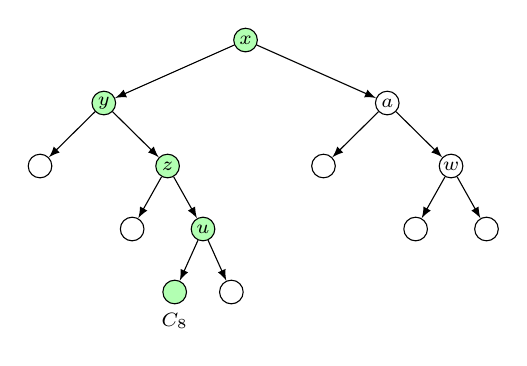
\begin{tikzpicture}[>=latex, xscale = 0.9]
    
    \node[inner, fill = green!30] (a) at (0, 0) {\scriptsize $x$};
    \node[inner, fill = green!30] (b) at (-2, -0.8) {\scriptsize $y$};
    \node[inner] (c) at (2, -0.8) {\scriptsize $a$};
    \node[inner] (d) at (-2.9, -1.6) {};
    \node[inner, fill = green!30] (e) at (-1.1, -1.6) {\scriptsize $z$};
    \node[inner] (f) at (1.1, -1.6) {};
    \node[inner] (g) at (2.9, -1.6) {\scriptsize $w$};

    \node[inner] (h) at (-1.6, -2.4) {};
	\node[inner, fill = green!30] (i) at (-0.6, -2.4) {\scriptsize $u$};
    
    \node[inner] (j) at (2.4, -2.4) {};
    \node[inner] (k) at (3.4, -2.4) {};

    \node[inner, fill = green!30] (l) at (-1, -3.2) {};
    \node[below = 4pt] at (l) {\scriptsize $C_{8}$};
    \node[inner] (m) at (-0.2, -3.2) {};
    
    \draw[ed] (a) -- (b);
    \draw[ed] (a) -- (c);
    \draw[ed] (b) -- (d);
    \draw[ed] (b) -- (e);
    \draw[ed] (c) -- (f);
    \draw[ed] (c) -- (g);
    \draw[ed] (e) -- (h);
    \draw[ed] (e) -- (i);
    \draw[ed] (g) -- (j);
    \draw[ed] (g) -- (k);
    \draw[ed] (i) -- (l);
    \draw[ed] (i) -- (m);
\end{tikzpicture}
    \end{minipage}
    \pause
    \begin{minipage}{0.4\linewidth}
        \centering
        $\frac{A \lor x ~~~ B \lor \neg x}{A \lor B} ~~~~~ \frac{A}{A \lor z}$
        \begin{itemize}
            \item Node $\Rightarrow$ disjunction of negations of queries.
            \item $(x \lor \neg y \lor \neg z \lor u)$.
        \end{itemize}
    \end{minipage}

\end{frame}

\begin{frame}{Corollaries}

    \begin{itemize}
        \item{} Running time of $\DPLL$ on $\PHP_{n}^{n + 1}$ is at least $2^{\Omega(n)}$.
            \pause
        \item{} [Alekhnovich, Hirsch, Itsykson 05; \alert{informal}] Running time of \alert{restricted}
            $\DPLL$ on some \alert{sat. formulas} is at least $2^{\Omega(n)}$. 
    \end{itemize}

    \pause
    \vspace{0.5cm}
    \begin{block}{Remark}
        $\alg{CDCL} \approx$ general resolution.
    \end{block}

    \pause
    \begin{itemize}
        \item{} Running time of $\alg{CDCL}$ on $\PHP_{n}^{n + 1}$ is at least $2^{\Omega(n)}$.
        \item{} \alert{Open problem}: what about sat. formulas and $\alg{CDCL}$?
    \end{itemize}

\end{frame}
        
    \end{center}

    
	\pause
    \pause
    \pause
    \pause
    \pause
    \begin{itemize}
        \item Heuristic $\mathbf{A}$ chooses a variable for splitting.
    	\pause
	    \item Heuristic $\mathbf{B}$ chooses the first value.
    	\pause
    	\item Simplification rules: \alert{no simplifications!}
    \end{itemize}
\end{frame}

\begin{frame}{$\DPLL$ and Resolution}
    
    \begin{theorem}
        $\DPLL$ algoritm makes $t$ splitting on \alert{unsatisfiable} CNF formula
        $$\varphi \coloneqq \bigwedge\limits_i C_i$$
        $\Rightarrow$ there exists a resolution proof of $\varphi$ of size $2t$.
    \end{theorem}

    \pause

    \begin{minipage}{0.58\linewidth}
        \centering
        \tikzstyle{inner} = [circle, minimum size = 0.3cm, draw, inner sep = 0.1pt]
\tikzstyle{gstyle} = [fill = green]
\tikzstyle{rstyle} = [fill = red]
\tikzstyle{ed} = [->, draw]
\tikzstyle{ops} = [alt=<{#1-}>{opacity = 1}{opacity = 0}]
\tikzstyle{opstyle} = [inner, ops = #1]
\tikzstyle{oped} = [ed, ops = #1]
\tikzstyle{gstyle} = [alt=<{#1}>{fill = green}{}]
\tikzstyle{rstyle} = [alt=<{#1}>{red!90!black}{}]
\tikzstyle{snakestyle} = [
    alt=<{#1}>{
        decorate,
        decoration = {
            snake,
            amplitude = 0.4mm,
            segment length = 2mm,
            post length = 1mm
        }
    }{}]


    
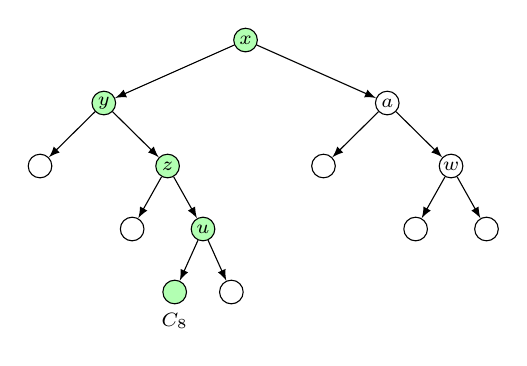
\begin{tikzpicture}[>=latex, xscale = 0.9]
    
    \node[inner, fill = green!30] (a) at (0, 0) {\scriptsize $x$};
    \node[inner, fill = green!30] (b) at (-2, -0.8) {\scriptsize $y$};
    \node[inner] (c) at (2, -0.8) {\scriptsize $a$};
    \node[inner] (d) at (-2.9, -1.6) {};
    \node[inner, fill = green!30] (e) at (-1.1, -1.6) {\scriptsize $z$};
    \node[inner] (f) at (1.1, -1.6) {};
    \node[inner] (g) at (2.9, -1.6) {\scriptsize $w$};

    \node[inner] (h) at (-1.6, -2.4) {};
	\node[inner, fill = green!30] (i) at (-0.6, -2.4) {\scriptsize $u$};
    
    \node[inner] (j) at (2.4, -2.4) {};
    \node[inner] (k) at (3.4, -2.4) {};

    \node[inner, fill = green!30] (l) at (-1, -3.2) {};
    \node[below = 4pt] at (l) {\scriptsize $C_{8}$};
    \node[inner] (m) at (-0.2, -3.2) {};
    
    \draw[ed] (a) -- (b);
    \draw[ed] (a) -- (c);
    \draw[ed] (b) -- (d);
    \draw[ed] (b) -- (e);
    \draw[ed] (c) -- (f);
    \draw[ed] (c) -- (g);
    \draw[ed] (e) -- (h);
    \draw[ed] (e) -- (i);
    \draw[ed] (g) -- (j);
    \draw[ed] (g) -- (k);
    \draw[ed] (i) -- (l);
    \draw[ed] (i) -- (m);
\end{tikzpicture}
    \end{minipage}
    \pause
    \begin{minipage}{0.4\linewidth}
        \centering
        $\frac{A \lor x ~~~ B \lor \neg x}{A \lor B} ~~~~~ \frac{A}{A \lor z}$
        \begin{itemize}
            \item Node $\Rightarrow$ disjunction of negations of queries.
            \item $(x \lor \neg y \lor \neg z \lor u)$.
        \end{itemize}
    \end{minipage}

\end{frame}

\begin{frame}{Flow formulas}
    \begin{minipage}{0.5 \linewidth}
        \tikzstyle{undir} = [thick]
\tikzstyle{dir} = [thick, ->, bend left = 10]
\tikzstyle{ver} = [thick, ->, draw, circle]

\begin{tikzpicture}[black, >=latex]
    \node[ver] (A) at (0, 0) {};
    \node[ver] (B) at (1.9, 1.9) {};
    \node[ver] (C) at (3, 0) {};
    \node[ver] (D) at (4, 1.2) {};
    \node[ver] (E) at (3.3, 3.7) {};
    \node[ver] (F) at (-0.5, 3) {};
    \node at (0, -0.2) {};

    \only<1>{
        \draw[undir] (A) to (B);
        \draw[undir] (A) to (C);
        \draw[undir] (B) to (C);
        \draw[undir] (C) to (D);
        \draw[undir] (B) to (D);
        \draw[undir] (D) to (E);
        \draw[undir] (E) to (F);
        \draw[undir] (F) to (A);
        \draw[undir] (B) to (F);
    }
    
	\only<2->{
        \draw[dir] (A) to (B);
        \draw[dir] (A) to (C);
        \draw[dir] (B) to (C);
        \draw[dir] (C) to (D);
        \draw[dir] (B) to (D);
        \draw[dir] (D) to (E);
        \draw[dir] (E) to (F);
        \draw[dir] (F) to (A);
        \draw[dir] (B) to (F);

        \draw[dir] (B) to (A);
        \draw[dir] (C) to (A);
        \draw[dir] (C) to (B);
        \draw[dir] (D) to (C);
        \draw[dir] (D) to (B);
        \draw[dir] (E) to (D);
        \draw[dir] (F) to (E);
        \draw[dir] (A) to (F);
        \draw[dir] (F) to (B);
    }
\end{tikzpicture}

        \putpos{15}{100}{
\includegraphics[scale = 0.1]{pics/utia-duck.png}}
    \end{minipage}%
    \begin{minipage}{0.5 \linewidth}
        \pause
        \pause
        \begin{itemize}
            \item $v\colon ~ \sum\limits_{e \in E^{\mathrm{in}}_v} x_{e} -
                \sum\limits_{e \in E^{\mathrm{out}}_v} x_{e} = c(v)$ 
                \textcolor{red}{$(\mathbb{R})$};
            \item $\sum\limits_{v} c(v) = 1$ \textcolor{red}{$(\mathbb{R})$};
            \item graph degree: $d$.
        \end{itemize}
    \end{minipage}

    \pause
    \vspace{0.2cm}
    \begin{itemize}
        \item{} There is an efficient Nullstellensatz proof of $\Flow$.
        \item{} [Alekhnovich, Razborov 03] If $G$ is an $(n, d, \alpha)$-expander $\Rightarrow$ any
            resolution proof has size $2^{\Omega(n)}$.
    \end{itemize}

    \pause

    \begin{corollary}[G\"{o}\"{o}s, Kamath, Robere, S 19]
        There is a monotone function in $\NC_2$ that cannot be computed by subexponential monotone
        circuits.
    \end{corollary}

\end{frame}